\colorlet{punct}{red!50!black}
\definecolor{background}{HTML}{F3F6FF}
\definecolor{delim}{RGB}{20,105,176}
\colorlet{numb}{magenta!50!black}

\lstdefinelanguage{json}{
	basicstyle=\normalfont\ttfamily,
	numberstyle=\scriptsize,
	stepnumber=1,
	numbersep=6pt,
	showstringspaces=false,
	breaklines=true,
	frame=lines,
	backgroundcolor=\color{background},
	literate=
	*{:}{{{\color{punct}{:}}}}{1}
	{,}{{{\color{punct}{,}}}}{1}
	{\{}{{{\color{delim}{\{}}}}{1}
	{\}}{{{\color{delim}{\}}}}}{1}
	{[}{{{\color{delim}{[}}}}{1}
	{]}{{{\color{delim}{]}}}}{1},
}


\chapter{Sincronización de Resultados}

\label{chapA:rest-api}

En este anexo, se proporcionan detalles adicionales los servicios RESP para realizar, incluyendo ejemplos y relación entre los recursos.

El servicio se comprende de dos recursos \textit{Collaborativefeature} y \textit{Collaborativesession}, el primero de estos representa la colección de los 15 feature calculados de una ventana de tiempo, y por otro lado la session de una actividad realizada por el individuo, la cual incluye una lista de features, como se esquematiza en la siguiente figura.

\begin{figure}[!htbp]
	\centering
	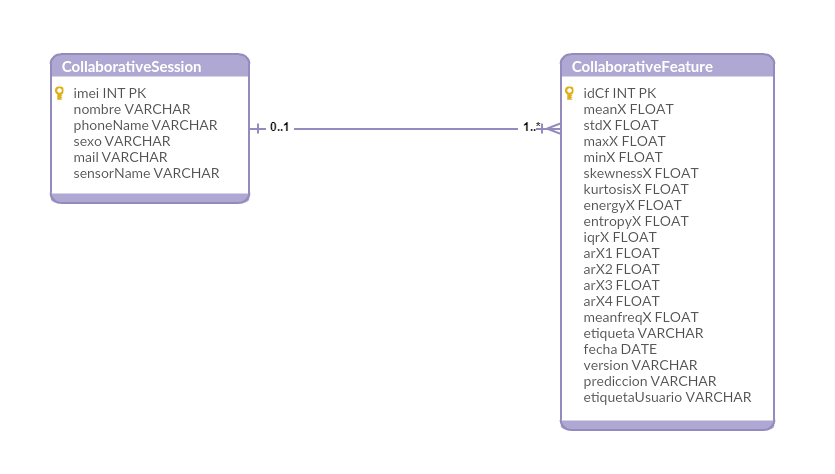
\includegraphics[width=0.7\linewidth]{anexos/der}
	\caption[Modelo de Datos]{\label{fig:der}Modelo de Datos}
\end{figure}

Los datos de la API publicada son las siguientes:

\textit{\textbf{http://[URL:PUERTO]/[CONTEXTO]/[RECURSO]/}}

Estando publicadas para las pruebas:

\begin{itemize}
	\item URL:PUERTO: ec2-52-27-63-54.us-west-2.compute.amazonaws.com:8080
	\item Contexto: ARrecolector
\end{itemize}



\section{Recurso CollaborativeSession}

POST para crear una session de entrenamiento \textit{ARrecolector/webresources/com.fpuna.entities.collaborativesession/}

\subsection{Request}

\begin{lstlisting}[language=json,firstnumber=1]
{
  "imei": "1234567890",
  "nombre": "Juan 123",
  "phoneName": "S33 mini",
  "sexo": "m",
  "mail": "soyunmailloco@gmail.com",
  "edad": "22",
  "sensorName": "Acelerometro XYZ",
  "collaborativefeatureList": [
     {
       "arX1": 0,
       "arX2": 0,
       "arX3": 0,
       "arX4": 0,
       "energyX": 0,
       "entropyX": 0,
       "etiqueta": "WALKING",
       "fecha": "2015-12-23T02:33:24-02:00",
       "idCf": 3,
       "iqrX": 0,
       "kurtosisX": 0,
       "maxX": 0,
       "meanX": 0,
       "meanfreqX": 0,
       "minX": 0,
       "skewnessX": 0,
       "stdX": 0,
       "version": "1.0",
       "prediccion": "S",
       "etiquetaUsuario": "STILL"
     }
  ]
}
\end{lstlisting}

\subsection{Response}

\section{Recurso CollaborativeFeature}

\subsection{Request}

\subsection{Response}